%% Obtained sig-alternate from http://www.acm.org/publications/proceedings-template
% This is compatible with acm_proc_article-sp
\documentclass[a4paper,twoside]{article}

\usepackage{graphicx}
\usepackage{url}
\usepackage[usenames]{color}
\usepackage{listings}
\usepackage{flushend}
\usepackage{dirtytalk}
\usepackage[lined]{algorithm2e}
\usepackage{epsfig}
\usepackage{subfigure}
\usepackage{calc}
\usepackage{amssymb}
\usepackage{amstext}
\usepackage{amsmath}
\usepackage{amsthm}
\usepackage{multicol}
\usepackage{pslatex}
\usepackage{apalike}
\usepackage{SCITEPRESS}
\pagenumbering{arabic}

\subfigtopskip=0pt
\subfigcapskip=0pt
\subfigbottomskip=0pt

\begin{document}

\title{Limited Use Cryptographic Tokens in Securing Ephemeral Cloud Servers}

\author{\authorname{Gautam Kumar, Brent Lagesse}
\affiliation{University of Washington Bothell, \break
Computing and Software Systems, \break
Bothell WA, \break USA}
\email{\{gautamk, lagesse\}@uw.edu}}


\keywords{Security, Moving Target Defence, Cryptography, Cloud Architecture}

\abstract{Many enterprises and consumers today are dependent on services deployed on Infrastructure as a Service (IaaS) cloud providers. Such cloud deployments can have hundreds of virtual servers running. Each virtual server needs to have access to sensitive information such as database passwords and API keys. In such as scenario, verifying that a large number of servers have not been compromised is an arduous task. In this paper we propose an architecture which limits the extent to which an attacker can exploit a compromised server in a large scale cloud deployment. To achieve such a limitation we propose the use of hash chains as an authentication mechanism for virtual server with a Central Trusted Authority (CTA) acting as a proxy to sensitive resources. This architecture shifts the requirement of security validation from hundreds of public facing servers to a few servers without public interfaces which comprise the CTA. Since hash chains offer an inherent limitation in their use, our architecture leans towards using ephemeral virtual servers, thus also providing a moving target defence.}

\onecolumn \maketitle \normalsize \vfill

\section{Introduction}

According to Microsoft \cite{harms_economics_2010}, more than 85\% of work done by enterprise IT departments is towards infrastructure maintenance. Cloud providers offer enterprises a unique advantage by minimizing the effort needed to purchase and maintain physical hardware.  %As a result, enterprises now consider hosting their infrastructure with cloud providers as a necessity rather than merely a competitive advantage \cite{mcafee_what_2011}.
%I removed "so" because I didn't really see how the previous sentence would lead me to conclude the sentence about increasing the attacker's cost.
Hosting infrastructure on the cloud comes with its own set of unique challenges and one of the primary concerns is security. Many cloud providers offer computational and storage resources on virtualized shared hardware to maximize utilization. The essence of securing cloud systems is using multiple layers \cite{panwar_layered_2011} of security to increase an attacker's cost for taking over the system. One of the emerging layers of security is the use of moving target defences \cite{evans_effectiveness_2011}.  
One of our focuses is to increase the cost to the attacker of launching a zero-day attack. According to Bilge \& Dumitras \cite{bilge_before_2012}, on average, zero day attacks remain undetected for 10 months. Once zero-day attacks are disclosed, malware authors begin to utilize them multiple orders of magnitude more frequently; however, there is often a significant delay between notification and the deployment of patches fixing the zero-day exploit. One of the goals of this project is to reduce the risk of systems when we are not aware of the existence of the vulnerability, but also during the gap of time that the community is made aware, but patches have not been fully deployed.

% Not sure what can be done to reduce the spacing between these paragraphs
% I've tried \par but it either seems to combine with the previous paragraph or have a large spacing

Consider the situation where a large service provider has a number of public facing servers with access to a private, remote database.  In the case that one of those public facing servers is compromised by an adversary, the data in the private database will be vulnerable for the entire duration that the attacker has access until the attack is detected and the vulnerable server patched or removed.  The goal of our work is to drastically reduce the length of time that the attacker has to sensitive information \textit{even when we do not know that the attack has occurred}. 

In this paper we propose an implementation of moving target defence using ephemeral servers and a central trusted authority which acts on behalf of an ephemeral server and proxies requests to sensitive resources such as database servers, caching servers and REST end points. Hash chains are used as an authentication mechanism by the central trusted authority. We take advantage of the limited use property of hash chains to authenticate ephemeral servers for a limited period of time. Hash chains are used as opposed to a timer as it reduces link-ability and provides cryptographic guarantees for its limited use.

\section{Background}
\textbf{Cloud infrastructure} today is characterised by three primary classes of products. Infrastructure as a Service or IaaS, Platform as a Service or PaaS and Software as a Service or SaaS. Our research in this paper is primarily focused on providing a mechanism to improve the security for organisations who use IaaS providers.  IaaS providers take on the responsibility of maintaining and securing physical hardware while organisations using IaaS are expected to maintain and secure their virtual hardware and also their application code. 

%
% PaaS providers such as Heroku and Google's AppEngine, offer services on top of an IaaS provider. PaaS providers assume the responsibility of maintaining and securing both physical and virtual hardware while the organisations assume the responsibility of merely securing application code. 
%
% SaaS providers offer complete applications hosted towards their customer's need and take on all the responsibility of maintaining and securing hardware and application code. 
%
%
%
% \subsection{Cryptographic hash function} 
% A cryptographic hash function is any one way function which meets the following requirements \cite{rogaway_cryptographic_2004} 
% \begin{itemize} 
% \item Preimage resistance
% \item Collision resistance
% \item Second Preimage resistance
% \end{itemize}
% 
% A hash function has preimage resistance if given a hash value $h$ it is computationally infeasible to find any message $m$ such that $h = hash(k,m)$ where $k$ is the hash key.
% 
% A hash function is collision resistant if, given two messages $m_{1}$ and $m_{2}$ it is hard to find a hash $h$ such that $h = hash(k,m_{1}) = hash(k,m_{2})$ where $k$ is the hash key.
% 
% A hash function has second pre-image resistance if given a message $m_{1}$ it is computationally infeasible to find a different message  $m_{2}$ such that $hash(k,m_{1}) = hash(k,m_{2})$ where $k$ is the hash key. The second pre-image resistance is a much harder property to achieve for hash functions. This property is closely related to the birthday problem \cite{lesser_exploring_1999}.
% 
% \begin{figure}[hbtp]
% 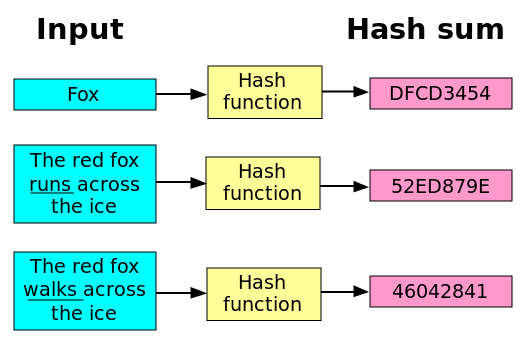
\includegraphics[scale=0.55]{hash_function.png}
% \caption{A simplified view of a hash chain where the start message is $K$ with $H$ being the cryptographic hash function. $H_1(K)$, $H_2(K)$ and $H_n(K)$ represent successive messages in the Hash chain  }
%\label{fig:hashchain}
%\end{figure}
%
\textbf{Hash Chains:}  Leslie Lamport \cite{lamport_password_1981} first proposed the use of hash chains in his paper on a method for secure password authentication over an insecure medium.  One of the properties of hash chain-based authentication is that it has a limited use lifespan.  We leverage this property in our system to limit the damage that any single compromised machine can cause.

%\say{A hash chain is a sequence of values derived via consecutive applications of a cryptographic hash function to an initial input. Due to the properties of the hash function, it is relatively easy to calculate successive values in the chain but given a particular value,it is infeasible to determine the previous value} 

%A hash chain in essence is merely the successive computation of a Cryptographic hash function on a given value as demonstrated in figure \ref{fig:hashchain}.

%As an example, Let $x$ be the initial password and $H$ be the cryptographic hash function.  A hash chain of length 2 would be $H^{2}(x) = H(H(x))$. A hash chain of $n$ values is denoted as $H^{n}(x)$ and the $i^{th}$ value in the chain would be computed as $x_{i} = H(x_{i-1})$.

%For a given value in the chain $x_{i}$ its computationally infeasible to determine the previous value in the chain $x_{i-1}$.

\textbf{Threats:}
According to OWASP, \say{Sensitive data exposure} is the one of the most critical types of security threat in web applications as of 2013 \cite{wichers_owasp_2014}. Sensitive data exposure refers to the unintended exposure of sensitive information such as passwords, social security numbers and date of birth. In the context of a cloud systems sensitive information may also include credentials to access a database, email server and REST API keys. These credentials are used to authenticate cloud servers with third party services within or outside the private cloud network. Credentials are usually stored as part of configuration files or in a server's memory. Such credentials have a very long life time and are sometimes valid of years. This increases the risk of data exposure when an attacker has a lengthy period of time within which they can discover and exploit such credentials.

A report by Risk Based Security \cite{risk_based_executives_2014} notes that the number of data leaks has dramatically increased from 2012 to 2013, to the tune of \$812 million. Leaking of credentials as mentioned earlier, could potentially grant access to malicious entities within protected environments such as a corporate network. Sensitive data exposure can also be a consequence of other threats such as cross site scripting (XSS) and Code Injection both of which are considered highly critical threats based on OWASP's classification \cite{wichers_owasp_2014}. 

\section{Proposed architecture}

Our proposed architecture consists of three primary components. The Client Facing Server (CFS), the Central Trusted Authority (CTA) and the Sensitive Resources that we're trying protect as shown in figure \ref{fig:architectureoverview}. 

\begin{figure*}[!ht]
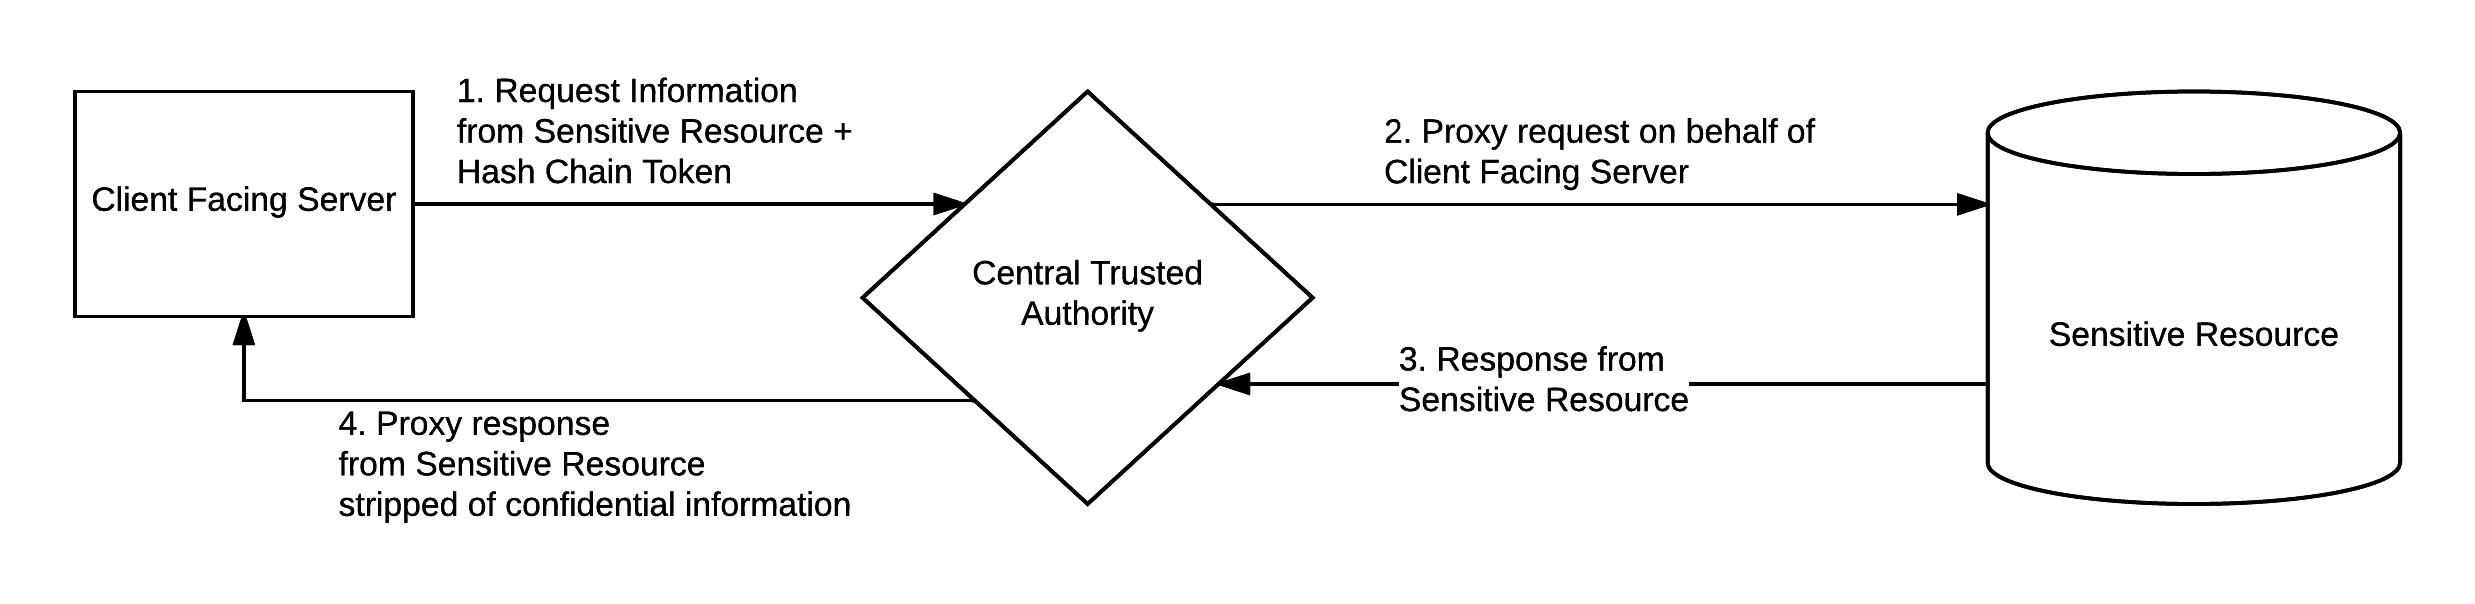
\includegraphics[keepaspectratio=true,scale=0.75]{overview_architecture.png}
\caption{Architectural overview of the system. This figure describes the three primary modules involved. The client facing server, The central trusted authority and a sensitive resource.}
\label{fig:architectureoverview} 
\end{figure*}

\emph{Client Facing Servers} are any servers which interact with entities on a public network such as Load balancers, reverse proxies and application servers. CFSs are assumed to be the most vulnerable to exploits by malicious entities. To offer moving target defence and increase the cost to an attacker, CFSs have a limited lifetime based on the length of the hash chain. When a hash chain expires the CFS is expected to shutdown because it can no longer authenticate itself with the CTA.

The \emph{Central Trusted Authority} is an entity within the corporate or private network which acts on behalf of a CFS when a sensitive resource is requested. To act on behalf of a CFS the CTA proxies requests to resources such databases and external APIs and includes authenticating information required by the resources. The authenticating information such as DB Passwords and API Keys are not available to CFS.  Because the CTA is not publicly available and there are orders of magnitude less CTAs in a system, it is assumed that the CTA is trustworthy as it will be easier to harden the system and monitor the limited types of activity on it.
The CTA verifies the identity of a CFS using a hash chain as explained in section \ref{sec:cta-architecture} and figure \ref{fig:ctaarchitecture} elaborates on the architecture of the CTA.

\begin{figure*}[!ht]
  \centering
  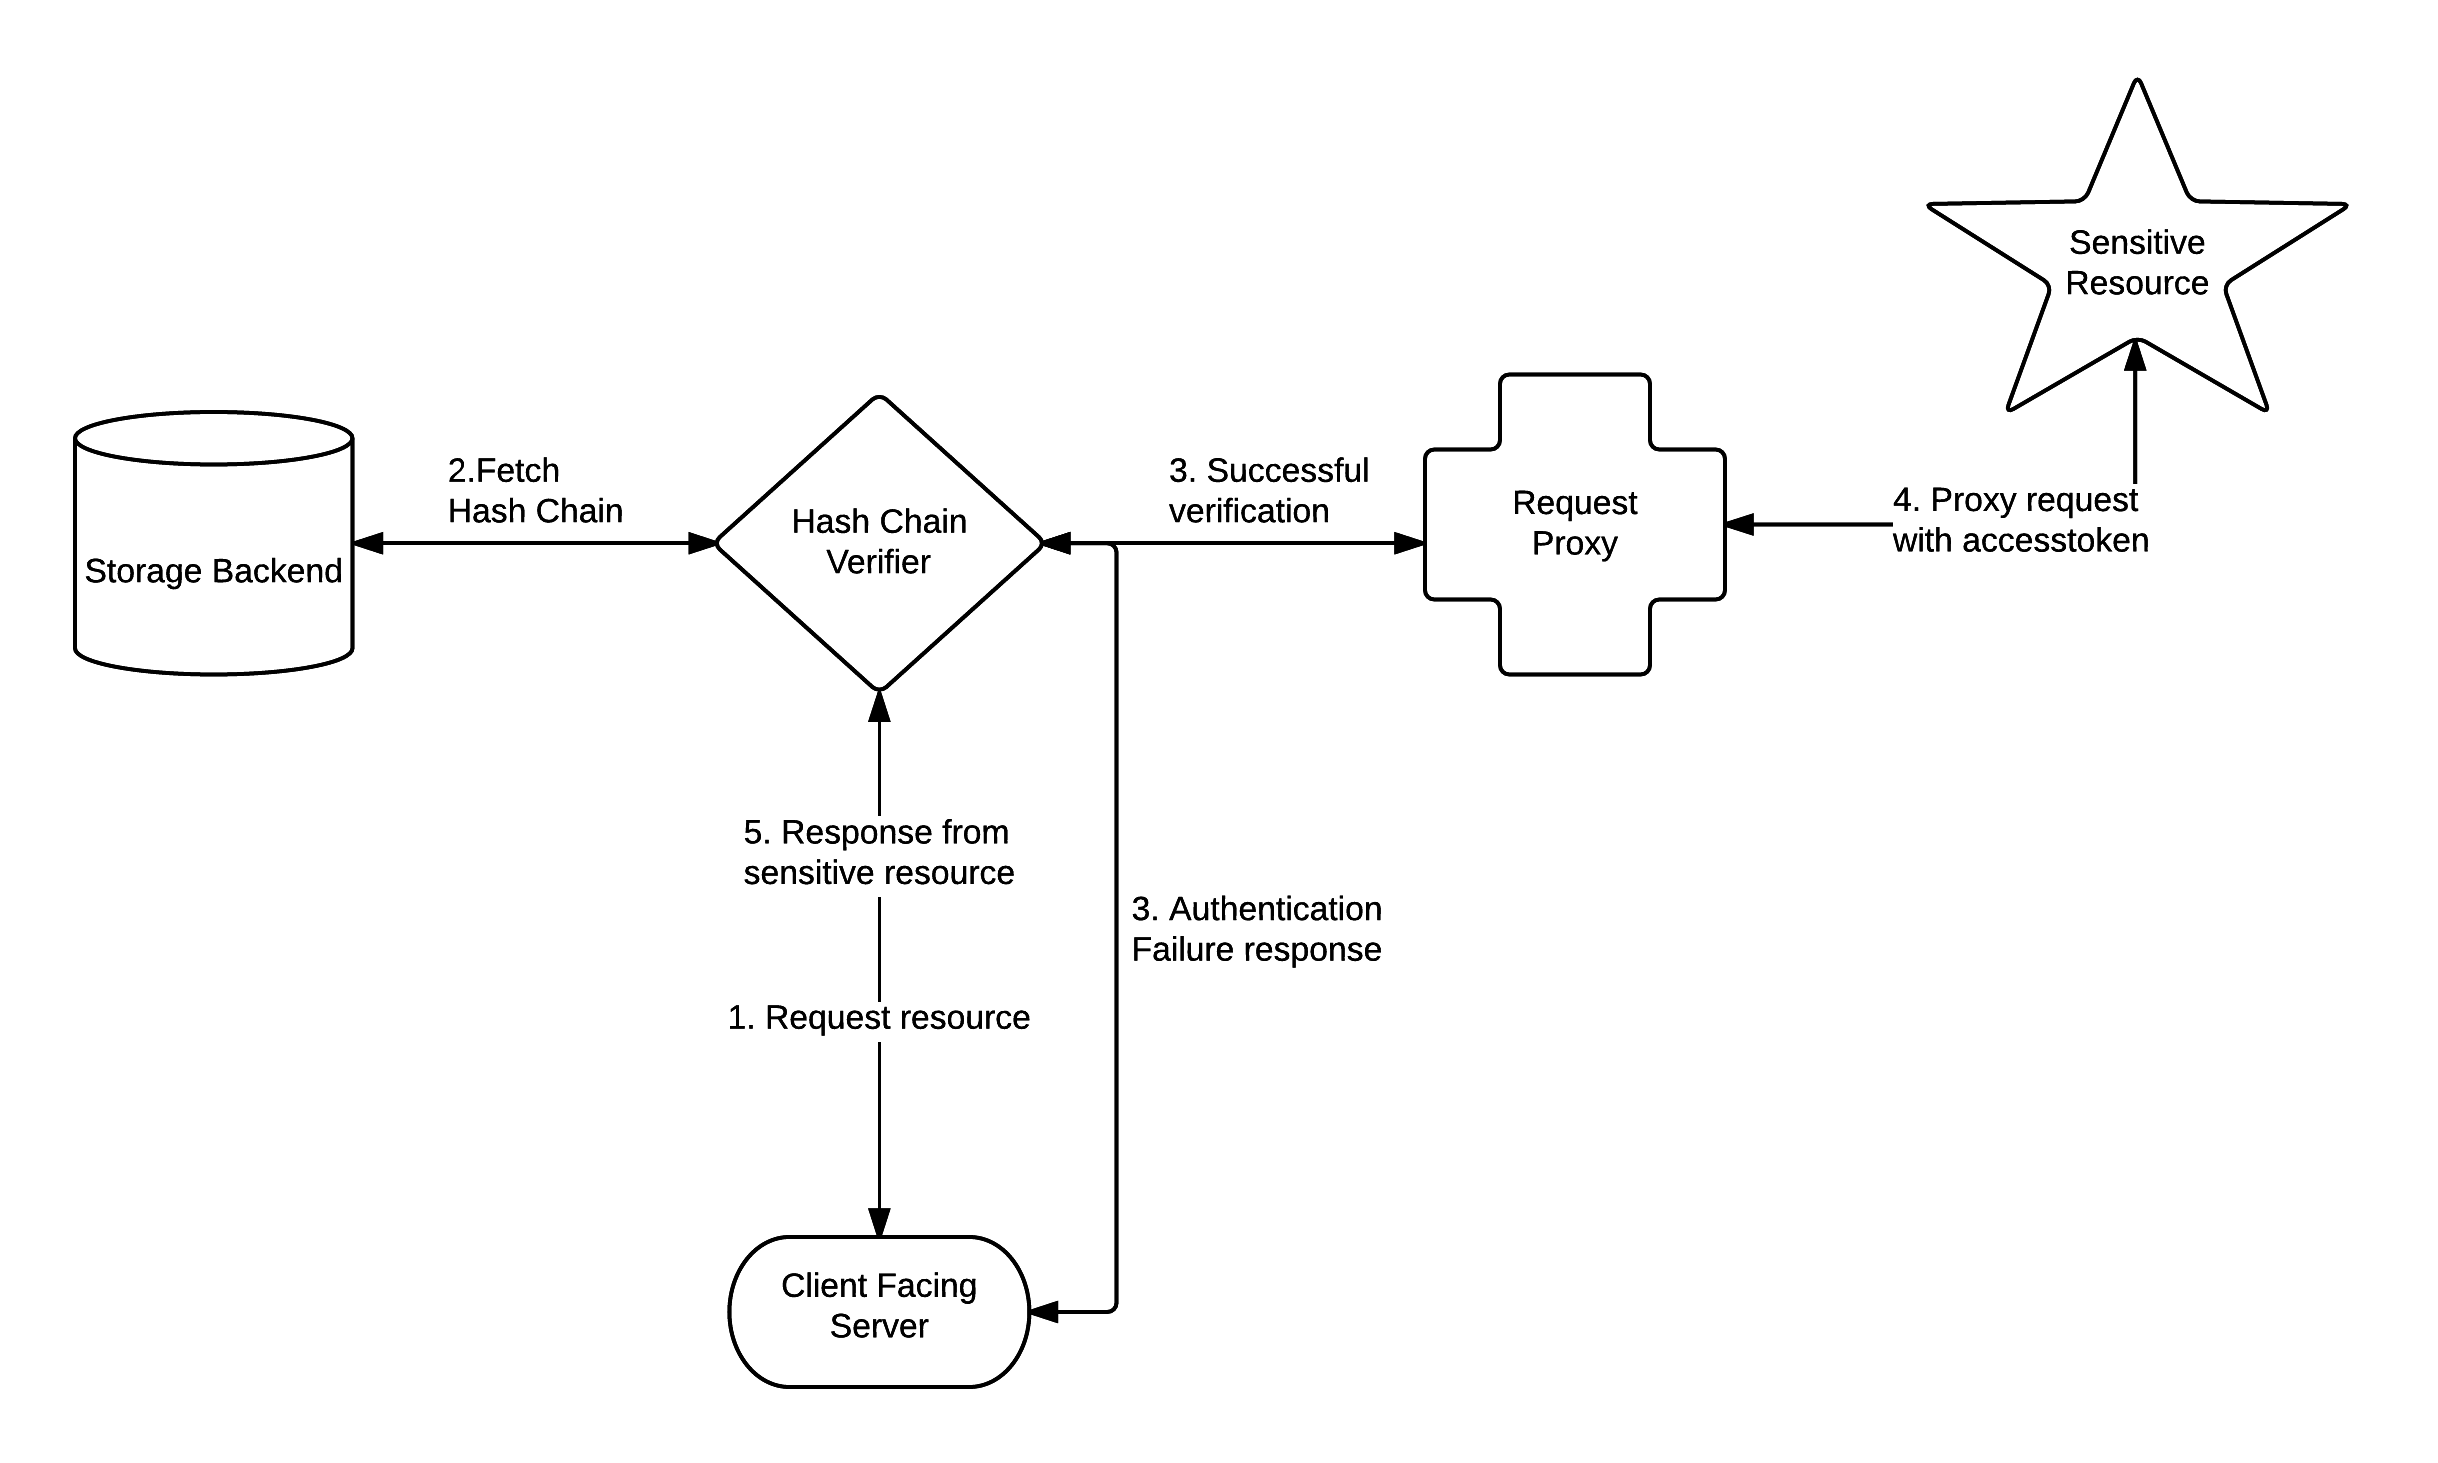
\includegraphics[keepaspectratio=true,scale=0.75]{cta_architecture}
  \caption{Architecture of the Central Trusted Authority. The CTA consists of a storage backend, a hash chain verifier and a request proxy.}
  \label{fig:ctaarchitecture}
\end{figure*}

 \subsection{Assumptions}


Client facing servers are the servers which are exposed outside the private cloud network environment. These client facing servers could potentially be load balancing servers, compute servers.
%
The client facing servers are assumed to be ephemeral. This is common in many cloud deployments \cite{vaquero_dynamically_2011} and contributes to the moving target nature of the security architecture. Companies such as Netflix expect this behaviour with their chaos engineering architecture \cite{basiri_chaos_2016}. This allows for higher reliability of their server infrastructure.
%
Client facing servers are expected to shut down after their hash chain expires. This contributes to the ephemeral nature and also to moving target defence of the overall system.


\subsection{CTA Architecture and Implementation} \label{sec:cta-architecture}

The Central Trusted Authority consists of three primary components, A hash chain verifier, A storage back-end and a request proxy. The CTA performs three roles within the system, which are

\begin{itemize}
\item Create new hash chains
\item Verify hash chains
\item Proxy requests to resources
\end{itemize}

\textbf{Creating a new hash chain:}
Hash chains are created by iteratively hashing a secret key $K$, $n$ number of times. 
After the hash chain is created the CTA stores $H^{n}(K)$ in the storage backend and returns $K$ and $n$ to the client facing server. The secret key $K$ is not stored by the CTA. The client facing server can now use the the secret key $n$ number of times. This process is detailed in Algorithm  \ref{algo_generating_hash_chain}.

\begin{algorithm}
\SetAlgoLined
\caption{Generating a Hash Chain}
\label{algo_generating_hash_chain}
\LinesNumbered
\KwData{Hash Chain secret $K$ and Hash chain length $N$}
\KwResult{Hash Chain $H^{N}(K)$}
$i \leftarrow 1 $\;
$H^{1}(K) \leftarrow H(K)$ \;
\While{$i <= N$}{
	$i\leftarrow i + 1$\;
	$H^{i}(K)\leftarrow H(H^{i-1}(K))$\;
}
\KwRet{$H^{i}(K)$ where $i$ equals $N$} \;
\end{algorithm}
\textbf{Hash chain verification:}
Hash chains are used to authenticate client facing server requests which require access to a sensitive resource. The hash chain verification is detailed in algorithm \ref{algo_hash_chain_verification}.

\begin{algorithm}
\SetAlgoLined
\caption{Verification of Hash Chain authentication}
\label{algo_hash_chain_verification}
\LinesNumbered
\KwData{Authentication key $H^{i-1}(K)$ from the client}
\KwResult{Response from sensitive resource}
	Let $H_{client}^{i} = H(H^{i-1}(K))$ \;
	Let $AuthenticationData = fetch(H_{client}^{i})$ \;
	
	\eIf{AuthenticationData exists in storage backend}{
		replace $H_{client}^{i}$ with $H^{i-1}(K)$ in storage backend \;
		fetch and return response from sensitive resource \;
	}{
		return authentication failure \;
	}
\end{algorithm}

\section{Performance}

\textbf{Hash chain creation:}
%\begin{figure}[h]
%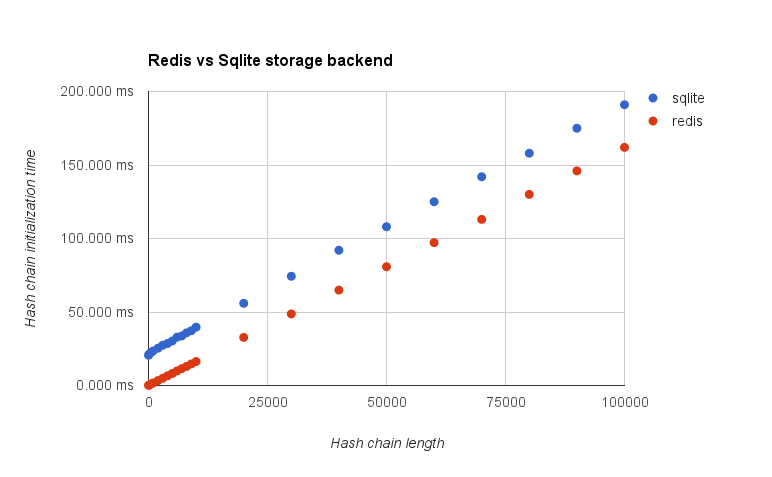
\includegraphics[width=\columnwidth]{performance}
%\caption{Linear time complexity of the hash chain initialization. Execution platform Intel i5-5200U 2.2Ghz, 12GB RAM, SHA-256 based on python 2.7}
%\label{fig:performance}
%\end{figure}
In our testing hash chain initialization showed a linear increase, $O(n)$, in time complexity based with hash chain length ($n$) . This is in line with our expectations for hash chain implementations.

In our proposed architecture hash chain length affects CFS uptime based on the equation,

\[
	Uptime = \frac{Hash\ chain\ length}{Requests\ per\  second} 
\]

where $Uptime$ is the maximum time in seconds that a CFS can effectively operate, $Hash\ chain\ length$ is the size of the hash chain provided to the CFS at startup while $Requests\ per\ second$ is the average number of requests that a CFS needs to make to a CTA.


\textbf{Hash chain verification and request proxy:}
Hash chain verification is a significantly faster process, $O(1)$, when compared to hash chain creation. Thus performance of the CFS is impacted merely by the delay introduced due to the request proxy. 

Our testing reveals that an additional delay in the range of $0.05$ to $0.15$ seconds is introduced by using Hash chain verification and a simple implementation of request proxy as illustrated by figures \ref{fig:verify_20s} and \ref{fig:direct_20s}.

\begin{figure}[h]
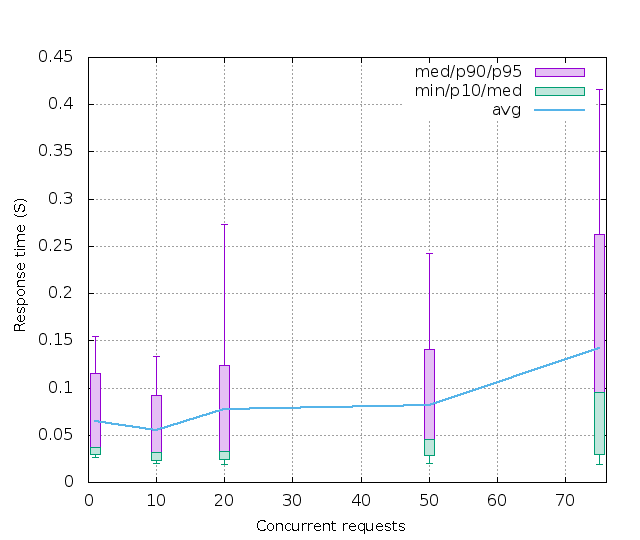
\includegraphics[width=\columnwidth]{verify_20s}
\caption{Response time for requests made to a resource through the CTA with a SHA-256 hash chain. The X-axis is the number of concurrent requests made and the Y-axis describes the response time in seconds}
\label{fig:verify_20s}
\end{figure}

\begin{figure}[h]
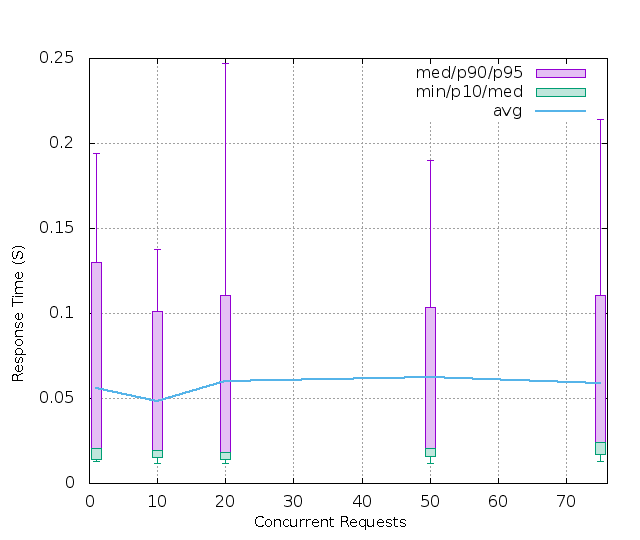
\includegraphics[width=\columnwidth]{direct_20s}
\caption{Response time for requests made to a resource directly without authenticating with the CTA. The X-axis is the number of concurrent requests made and the Y-axis describes the response time in seconds}
\label{fig:direct_20s}
\end{figure}

\textbf{Testing environment:}
Our testing environment was based in AWS. The CTA was a pool of EC2 machines behind a elastic load balancer. Load tests were conducted using multiple CFSs located in the same AWS region as the CTA. The payload requested by the CFS was a file located on S3.

\subsection{Server Pool}

Creating new virtual servers to act as CFSs can be a slow and expensive process; however, by creating a pool of unused CFSs to act as quick replacements, we can minimize delay for customers. The size of the CFS pool needs to be balanced based on the time to initialize a new virtual server, the size of the hash chain, and the rate at which requests are made.

The relationship between pool size, hash chain length and requests per second can be illustrated by equation \ref{eq:poolsize}.  

\begin{table}
	

\begin{center}
	\begin{tabular}{ | l | r |}
		\hline
		$n$ & Length of hash chain \\ \hline 
		$r_{req}$ & Request rate  \\ \hline
		$r_{boot}$ & Boot rate  \\ \hline
		$r_{pool}$ & Pool size change rate\\
		\hline
		
	\end{tabular}
	
	\label{tab:terms}
\end{center}
\caption{Table of terms for equation \ref{eq:poolsize}}
\end{table}

\begin{equation} 
 r_{pool} = r_{boot} - \frac{r_{req}}{n}
 \label{eq:poolsize}
\end{equation}
\begin{figure*}[!ht]
  \centering
  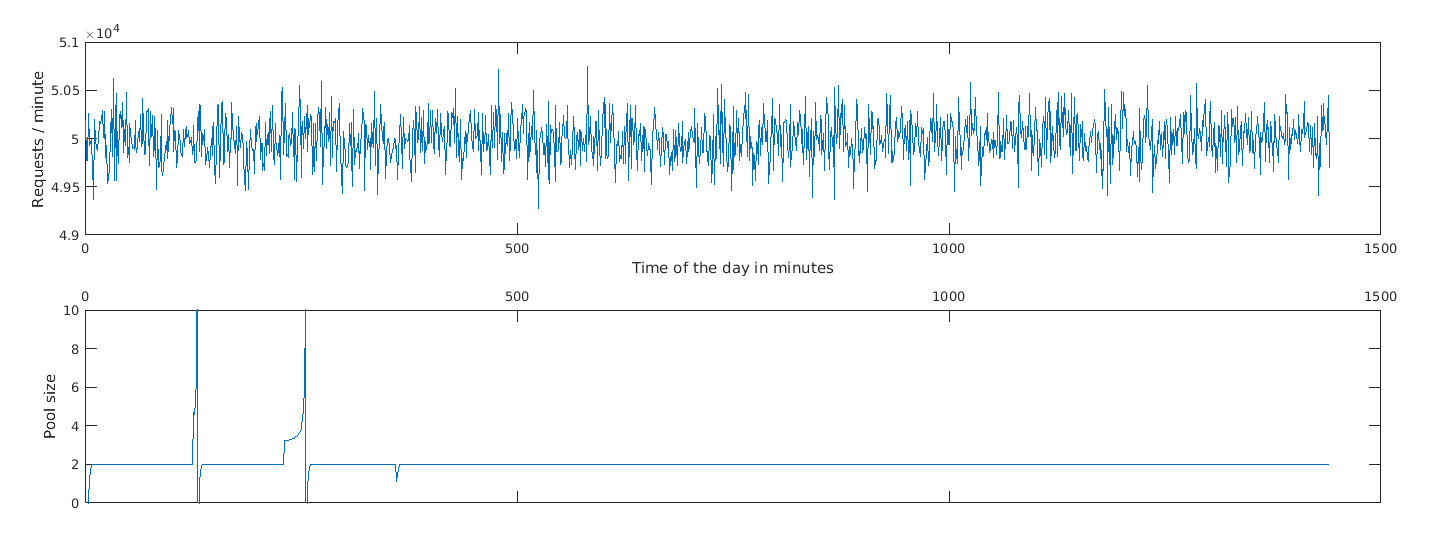
\includegraphics[keepaspectratio=true,scale=0.375]{poolsize}
\caption{The upper plot shows a random request rate generated by a poisson distribution is with a lambda of 50,000 and the lower plot describes the pool size based on equation \ref{eq:poolsize}}
\label{fig:poolsize}
\end{figure*}

Equation \ref{eq:poolsize} describes how the change in pool size relates to the length of the hash, the boot rate, and the request rate.   When the number of requests that have been authenticated using a hash chain reaches the length of the hash chain, the VM using it is no longer functional and must be shut down and replaced.  Our system keeps a pool of VMs in reserve so that this process is transparent to the user and no delay is noticed.  System designers can use this equation to minimize the number of VMs that have to be held in reserve to sufficiently handle a variable load over the course of time.  Boot rate is defined as the average number of VMs that can be instantiated in a particular period of time.  Request rate is the average number of requests that come in during a time period.  This value can change overtime as services will have different peak usage times during a day.   

As an example consider that a company receives 50,000 requests per minute on an average day.  They want to replace their VMs every 10 minutes, so each VM should have a hash chain with a length of 5000.   They would have to boot 1 VM every 5 minutes.  Figure \ref{fig:poolsize} shows how our system would keep a small pool of VMs that would not consume significant resources, but would also never run out when the request rates are sampled from a poisson distribution with a lambda of 50,000.

% In figure \ref{fig:poolsize} we show how the pool size can vary over time with a change in traffic patterns.  

Part of our future work is to design an adaptive algorithm that solves the multi-criteria optimization problem that manages the creating of new VMs based on learned traffic patterns.

\section{Security Threats}

The proposed architecture of using a Central Trusted Authority (CTA) to proxy requests on behalf of all the clients places the CTA as a single point of failure. We deem this an acceptable trade-off as the CTA is not a public facing system and only serves the purpose of verifying hash chains and proxying requests.  As a result, hardening its defences against possible threats becomes an easier problem.  In our current implementation, the CTA is a single hardened server; however, we are currently working on a distributed implementation.

Our architecture proposal does not prescribe any particular hardware / VM co-location for any components in the CTA. Thus each component can be implemented on separate machines or the CTA can be instantiated as a whole within a single VM. In this section we detail the potential security threats against each component and possible mitigation strategies.

\begin{figure*}[!ht]
  \centering
  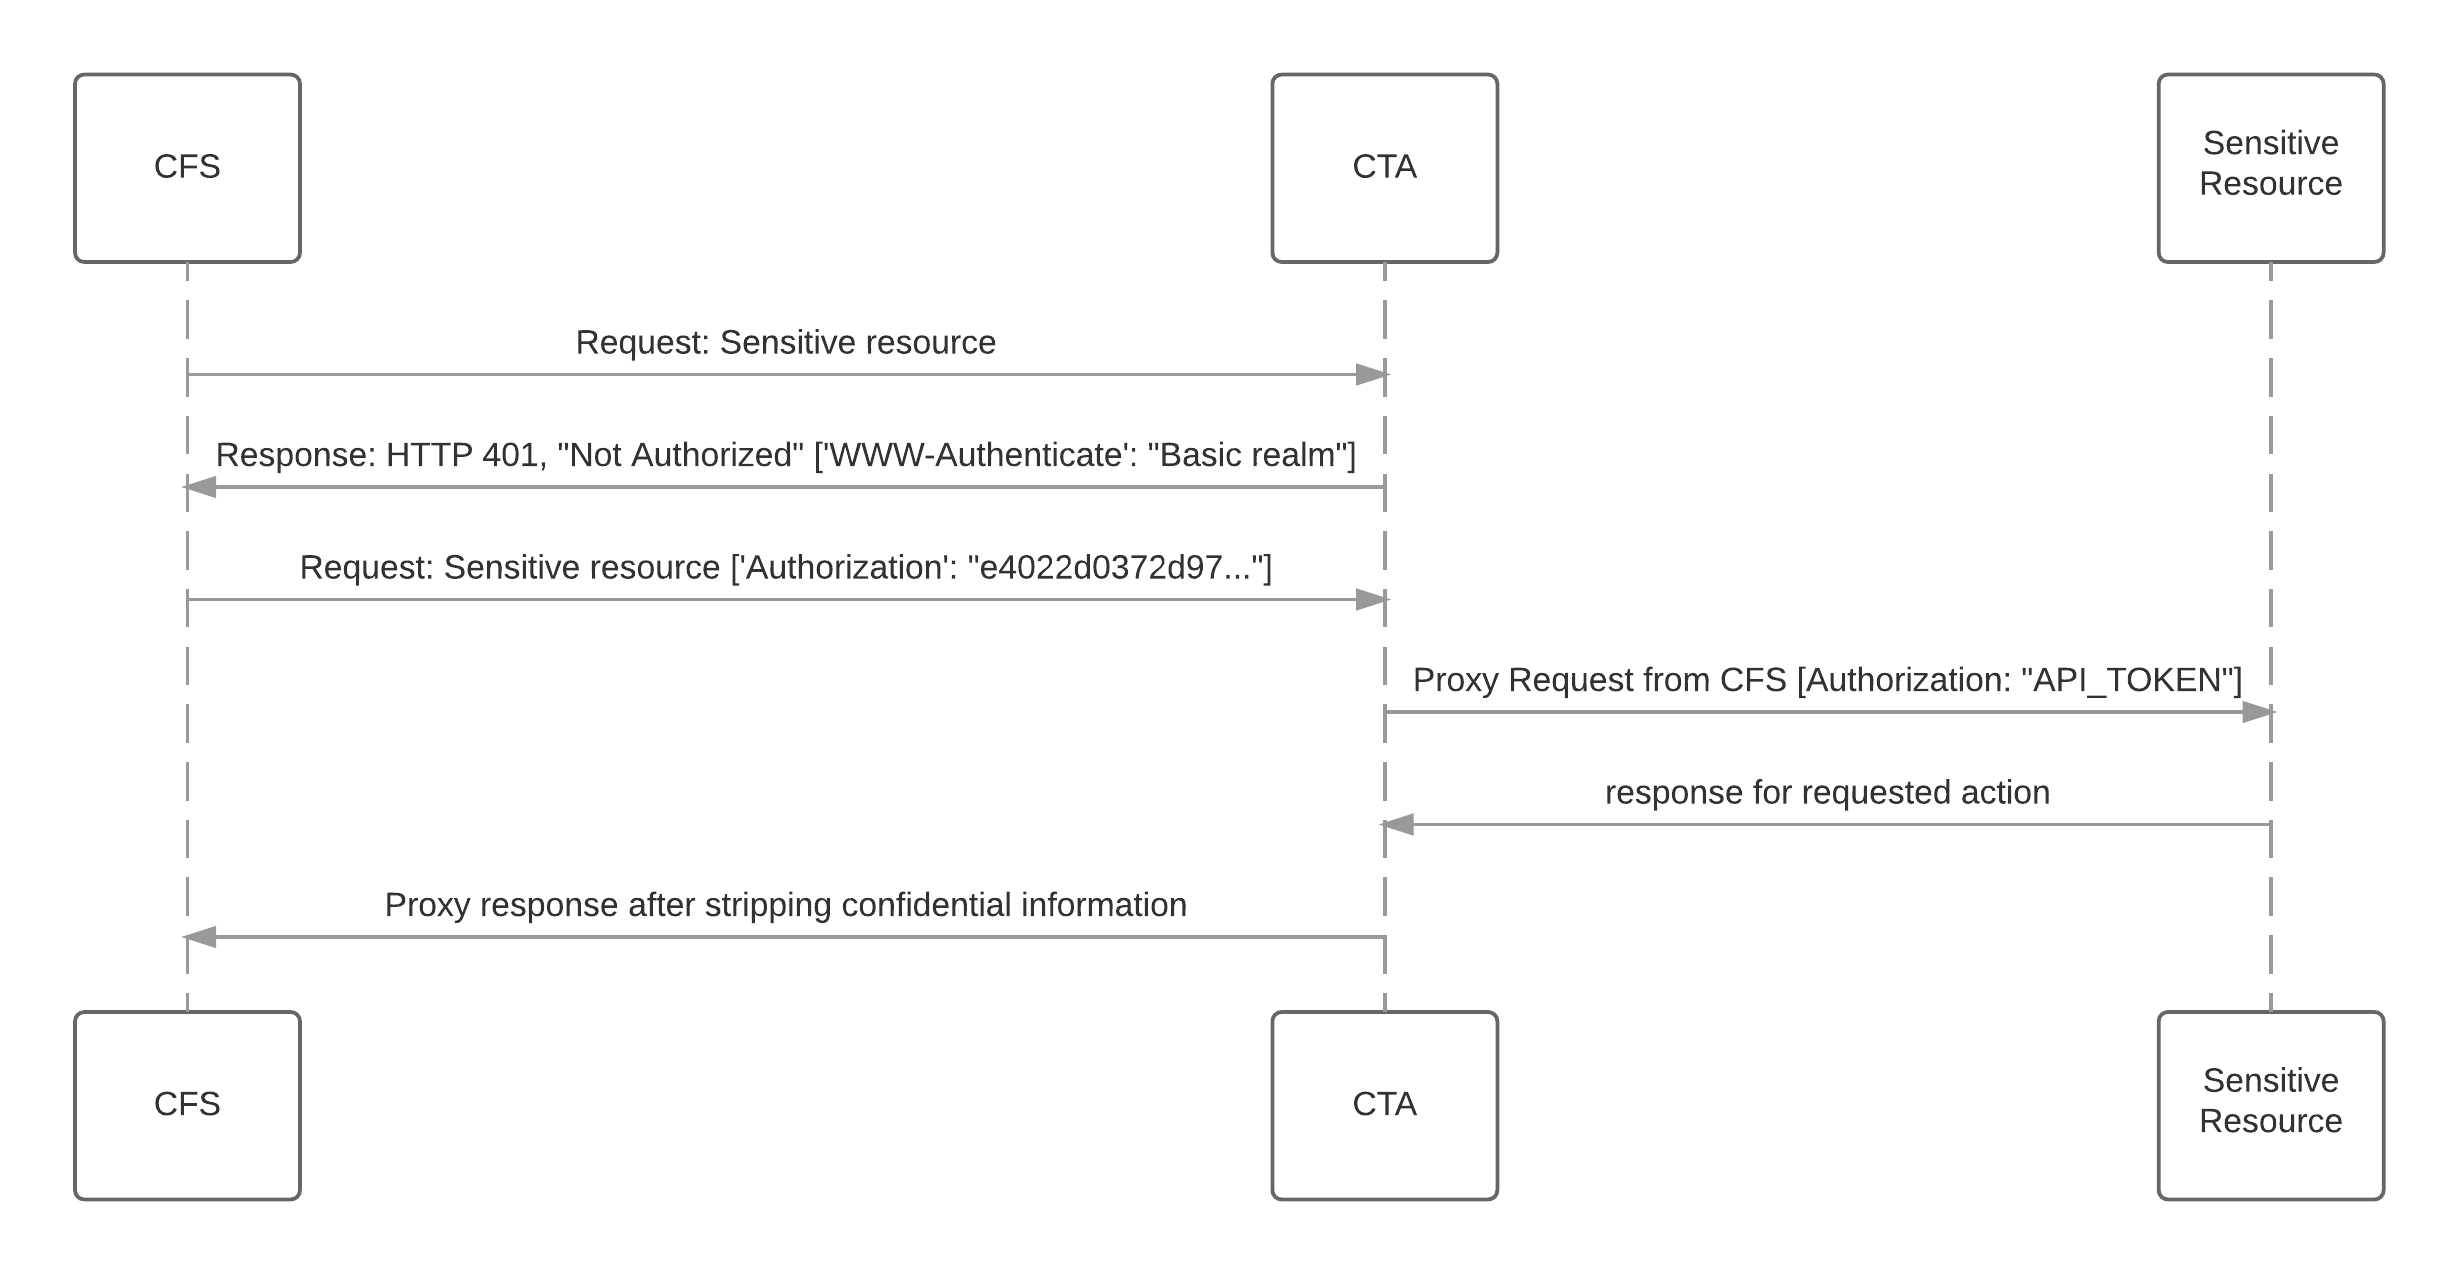
\includegraphics[keepaspectratio=true,scale=0.70]{sequence_diagram}
  \caption{Sequence diagram describing the authentication and proxying capabilities of the CTA. CFS refers to Client Facing Server while CTA refers to Central Trusted Authority}
  \label{fig:ctaarchitecture}
\end{figure*}
\subsection{Malicious Request Proxy}

The request proxy component acts on behalf of the client facing server to make a call to a sensitive resource such as an API endpoint. The request proxy is also responsible for attaching authentication information such as an API Key when contacting the API endpoint. Upon receiving a response from the sensitive resource the request proxy strips out sensitive information such as API Keys and Refresh Tokens before forwarding the response to the client facing server.  Under this threat scenario the request proxy is assumed to be untrustworthy and potentially malicious despite the our earlier argument that this case is unlikely.

Chen et al \cite{chen_towards_2012} propose a solution to this problem of a Malicious proxy using trusted hardware such as Trusted Platform Module (TPM) or the IBM 4758 cryptographic coprocessor \cite{parno_bootstrapping_2010}.  The CTA executable would also verified by a trusted third party to operate correctly as a proxy as described in \cite{parno_bootstrapping_2010}.

There are three primary attacks that a malicious actor may perform on the CTA. First, the attacker may try to expose the sensitive information stored, such as API keys and DB passwords, from the CTA using vulnerabilities in the CTA executable. Second, the attacker could potentially modify the requests / responses which are being proxied by the CTA. Third the attacker could potentially launch a reboot attack to inject a malicious executable after attestation to carry out one of the above attacks.

Prior work \cite{libert_tracing_2008} \cite{mccune_flicker_2008} on preventing reboot-attacks can be leveraged to impede the attacker's ability to inject a malicious executable. The proposed architecture also allows for the CTA to be placed behind secure corporate firewalls to further limit the risk of a malicious take over by an attacker. Further work is needed to fully secure the CTA against a malicious proxy.

%\subsection{Insecure Storage back-end}

%Our proposed architecture can accommodate various kinds of storage backends and thus potential security threats against the storage backend may vary. 

%Considering the scenario of an RDBMS system, The most common vulnerability is SQL Injection and a lot prior of work has been done to secure RDBMS systems against SQL Injection \cite{halfond_amnesia:_2005, boyd_sqlrand:_2004, halfond_classification_2006} and those techniques to drastically limit the risk of data leakage or system takeover.

%Using a pre-hardened database as a service such as Amazon's RDS or Google's CloudSQL can further improve the security of our storage backend \cite{curino_relational_2011} .

\section{Discussions}
\label{sec:future}
\subsection{Providing moving target defence}

Green et al \cite{green_characterizing_2015} identify Unpredictability, Vastness and Revocability as some of the criteria for evaluating moving target defences. In this section we try define how our implementation conforms to these criteria.

\textbf{Unpredictability:} Cryptographic hash functions \cite{rogaway_cryptographic_2004} are designed to be collision resistant and comply with the avalanche effect and thus the generated sequence is highly unpredictable in nature. Hash chains can compound this effect by sequential application of the cryptographic hash function.

\textbf{Vastness:} A secure cryptographic hash function such as SHA-256 has a vast state space as the output could be any of $2^{256}$ different values.  As a result, the likelihood of an attacker guessing the correct value is negligible.

\textbf{Revocability:} The proposed architecture allows individual chains or a group of chains to be revoked merely by purging them from the database. Further group / hierarchical revocability can be achieved using Merkle hash tree implementations as a means of Hash chain generation.

%\textbf{Limitations:}
%The proposed architecture and implementation is designed for cloud IaaS providers such as Amazon AWS where ephemeral servers are easily managed.  As a result, the proposed system is not extensible to a cloud provider without the ability to quickly provide large number of ephemeral servers  could result is significant performance degradation.


% Removing to fit within the 8 page limit
%\subsection{Artificial diversity}

%One concern of our system is that if an attacker is able to compromise one server, then once that server is destroyed, they will move on to another CFS.  For the case of some vulnerabilities, this will be true.  In those cases, we have at least raised the cost to the attacker as they will have to exploit the vulnerability over and over again.  This raises the chance that they will be detected, and if the exploit is costly, then it puts a greater strain on their resources.  In some applications, we will be able to implement automated diversity into the CFSs that will mitigate attacks even further.  Diversity in computer systems \cite{forrest_building_1997, littlewood_redundancy_2004, cox_n-variant_2006} has been studied to demonstrate its effectiveness at raising costs to attackers and we expect further research in the area to continue to improve the effectiveness of the defence we propose in this paper.  

%The proposed architecture lends itself well to establishing artificial diversity using a Distributed Hash Table to store the hash chains as suggested by Morell et al \cite{morrell_dht_2015}, thus further contributing to the un-predictability of the system and further limiting the risk introduced by a malicious node. 

\subsection{CTA Alternative}

In this paper we have presented our solution with a centralized CTA and argued that in some cases this approach is sufficient.  In the case that this solution does not work for an application, we are also exploring a DHT-based proxy though we have not yet implemented it.  In the DHT-based solution, there would be a large number of proxies in a DHT.  Each proxy in the DHT would be responsible for servicing a subset of requests from CFS.  In this solution, the DHT would be keyed on the hash chain hash value, so the requests would be routed to a different proxy every time.  By using a DHT-based solution, an adversary would only be able to compromise a subset of the requests, further limiting its ability to intercept targeted information or read widespread sensitive requests.  


\subsection{Future Work}

Formulating learning algorithms to create an adaptive balance between server lifespan and hash chain length to optimize computational resources in a cloud system, this can be derived from the equations we have derived in this paper and current work into load balancing in cloud systems \cite{randles_comparative_2010}. Such an adaptive system could be used to choose an ideal hash chain size and CFS pool in real time based on the performance requirements of a cloud system.

Timed Release Cryptography \cite{chalkias_timed_2006} can be integrated as a hash chain renewal mechanism to potentially increase the lifespan of a server after a certain cool off period. Implementing Time Release Cryptography would enable our architecture to accommodate systems where a constant pool of ephemeral servers are not available and existing servers can be populated with a batch of hash chains which can only be accessed after a certain period of time. 

A Merkle hash tree implementation middle-ware can potentially provide hierarchical authentication authorization capabilities to the CTA as illustrated by Yi \& Wang \cite{yi_cloud_2012}. In the scenario of an information leak, Merkle trees would allow administrators to black list either a single or a hierarchy of hash chains to safeguard the system.

%\subsection{Performance improvements}

%There are various avenues for performance improvements in our implementation, some of which are highlighted in this section. 

%Hash chain generation and verification is a well researched area. There have been various algorithms proposed to improve the performance of hash chain generation from O(n) time complexity to O(log n) \cite{coppersmith_almost_2002, 
%jakobsson_fractal_2002, kim_improved_2003, sella_computation-storage_2003, yum_single-layer_2009
%}. We plan to implement these algorithms to significantly improve the delay introduced by hash chain generation at CFS startup. Fischlin and Yum et al \cite{fischlin_fast_2004
%, yum_fast_2010
%} have proposed various techniques for improving performance of hash chain verification, implementing these techniques would enable our implementation to perform only a fraction of the work needed to perform hash chain verification thus reducing the delay introduced during CFS requests for a resource. 

%Our implementation is built in the python programming language, by taking advantage of the asynchronous event-driven programming paradigms we can significantly improve performance \cite{kinder_event-driven_2005} of our request proxy server. Other options to significantly improve performance include integrating into existing reverse proxy servers such as Apache, Nginx or HAProxy. These reverse proxy servers are written in C / C++ and migrating our implementation as a C module might also offer significantly performance improvements. 

\section{Related work}

There have been other systems proposed which offer moving target defence using a temporary address or a temporary authentication mechanism. Many technology companies have real world implementations of the Central Trusted Authority architecture similar to our proposal. In this section we present the most relevant proposals and discuss how our proposed architecture differs. 

Dunlop et al \cite{dunlop_mt6d:_2011} leverage the vast address space ($2^{128}$) of IPv6 to move the source and destination IP addresses mid-session based on a pre-agreed pattern to limit an attacker's ability to intercept or interfere with a TCP session. The technique proposed by Kampanakis \cite{kampanakis_sdn-based_2014}, however, operates at the network level by using an SDN's ability to vary the address space and the route taken by packets to increase the cost for an attacker and thus providing moving target defence.

Active authentication proposed by \cite{yiu_authentication_2011,aksari_active_2009,li_active_2014} offer a way to verify a user's identity based on their behaviour thus eliminating the need for hard to remember passwords. Active authentication is a form of moving target defence where the authenticating factor is constantly changing in a hard to predict manner, thus significantly increasing the cost for an attacker to reproduce the authenticating factor.

Confidant \cite{lyft_confidant:_2015} is a library maintained by Lyft, a transportation network company based out of San Francisco. Confidant provides an implementation of the Central trusted authority server with encryption at rest, authentication and authorization handled by AWS's Key Management Service, KMS and a storage backend of DynamoDB.  This system lacks the hash chain based approach that we use and as a result does not provide the additional moving target defence that raises the adversary's cost of launching an attack. Another limitation of this implementation is the inability to deploy a Confidant instance on a different cloud IaaS provider besides Amazon's AWS. 


\section{Conclusion}

In this paper we propose an architecture which increases the cost of exploiting vulnerabilities  for an attacker with minimal impact on performance by providing moving target defence using a pool of Client Facing Servers (CFS) which only operate for a relatively short period of time. Our architecture also significantly hampers an attacker's ability to steal sensitive configuration information from by centralizing configuration within a Central Trusted Authority.

We believe this approach can be used in cloud systems to limit the risk of a compromised client facing server.  Security-related software bugs are constantly being discovered and exploited, so while we may not be able to deploy a system that will never be compromised, we can deploy defences that limit the effectiveness of an attacker, even when they are utilizing a zero-day attack.

\section*{Acknowledgements}

The work presented in this paper was partially supported under US National Science Foundation Grant DGE-1419313. The author would like to thank Victoria Wettmarshausen from UW Bothell's Writing \& Communication Center for her feedback on the structure and presentation of this paper.

\bibliographystyle{apalike}
\bibliography{css539_class_see}


%\subsection{Reliability}
%
%A lot of research \cite{dutta_smartscale:_2012} \cite{vishwanath_characterizing_2010} \cite{xuejie_reliability_2013} \cite{kumar_dynamic_2012} has been conducted into improving the reliability of cloud systems through vertical, horizontal scaling and automatic provisioning. Much of that work can be leveraged for the purpose of improving the reliability of the proposed architecture. For example, Beltr{\'a}n \cite{beltran_automatic_2015} proposes an architecture of utilizing multi-tired load balancers to improve the reliability of a service. 
%
%Large scale database deployments typically deploy databases behind a reverse proxy for load balancing and Geo distribution \cite{hoff_7_2012}. Thus a reverse proxy such as Vitess \cite{hoff_7_2012} is ideally suited to act as the CTA in such architectures.

\end{document}




